\subsection{Abbildungen}
\begin{figure}[h]
	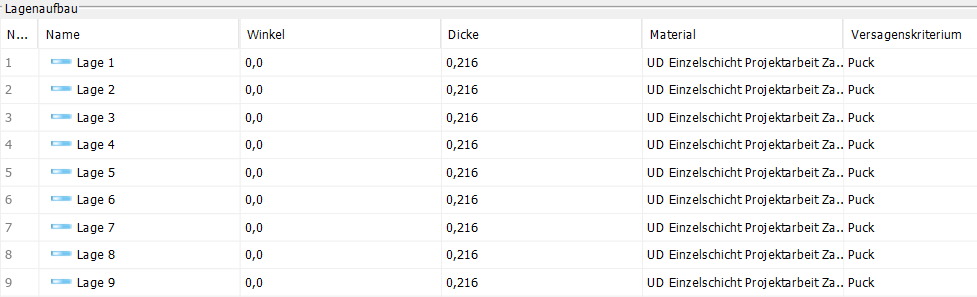
\includegraphics[width=1.0\textwidth]{Bilder/Lagenaufbau Holmgurte.png}
	\caption{Lagenaufbau Holmgurte}
	\label{fig:Lagenaufbau Holmgurte}
\end{figure}
\begin{figure}
	\includegraphics[width=1.0\textwidth]{Bilder/Lagenaufbau Steg dünn.png}
	\caption{Lagenaufbau Steg Bereich $III$}
	\label{fig:Lagenaufbau Steg dünn}
\end{figure}
\begin{figure}
	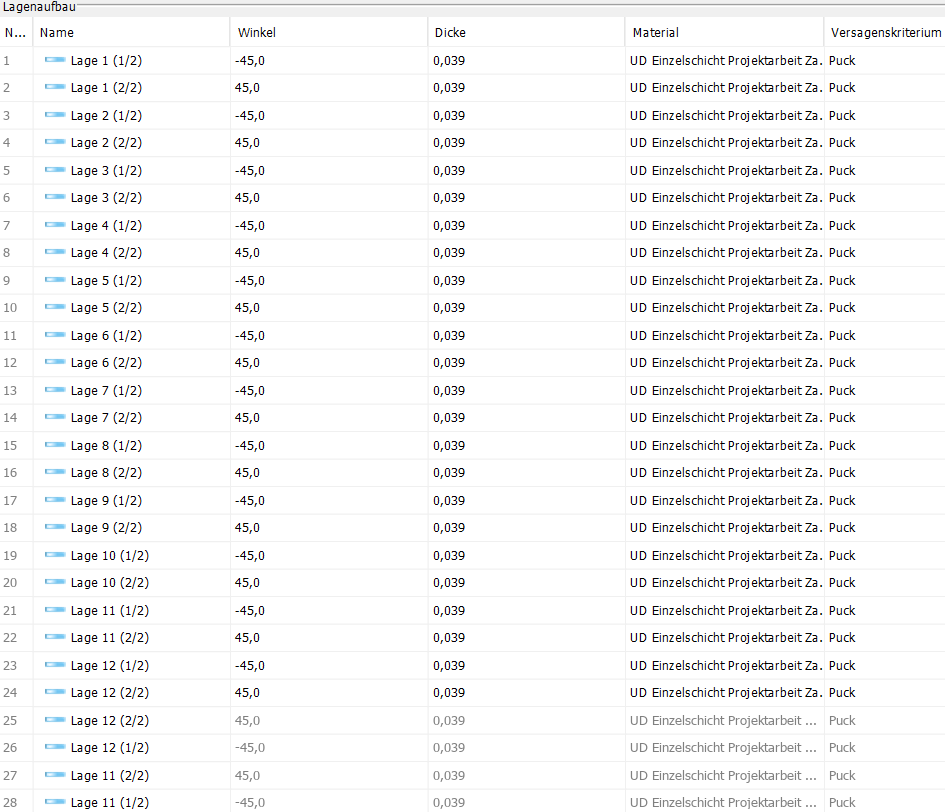
\includegraphics[width=1.0\textwidth]{Bilder/Lagenaufbau Steg dick.png}
	\caption{Lagenaufbau Steg Bereich $I$\&$II$}
	\label{fig:Lagenaufbau Steg dick}
\end{figure}
\begin{figure}
	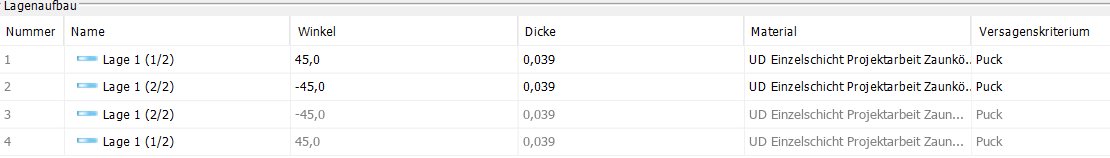
\includegraphics[width=1.0\textwidth]{Bilder/Lagenaufbau Haut.png}
	\caption{Lagenaufbau Flügelschale}
	\label{fig:Lagenaufbau Haut}
\end{figure}
\begin{figure}
	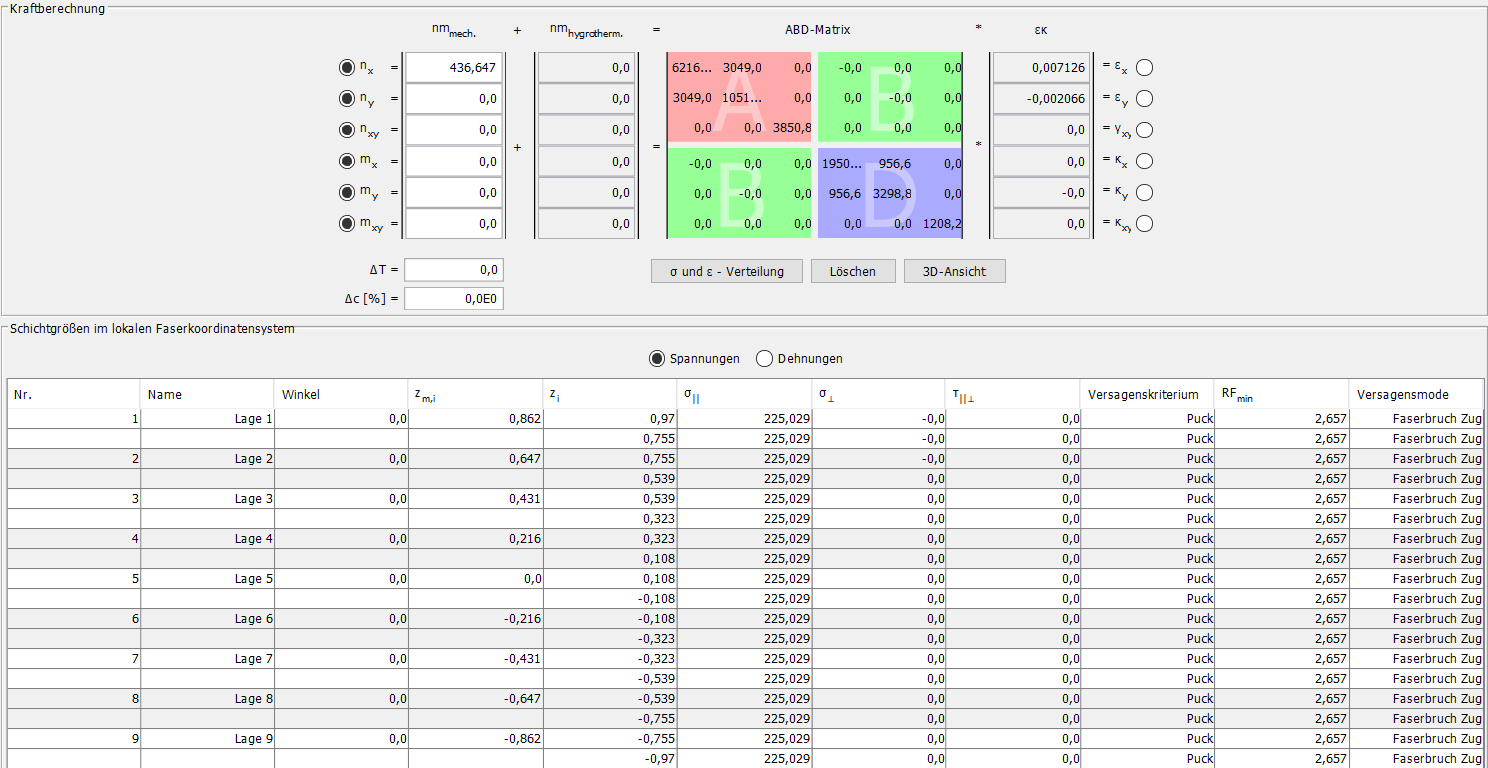
\includegraphics[width=1.0\textwidth]{Bilder/Berechnung Holmgurte.png}
	\caption{Berechnung Holmgurte}
	\label{fig:Berechnung Holmgurte}
\end{figure}
\begin{figure}
	\includegraphics[width=1.0\textwidth]{Bilder/Berechnung Steg dünn.png}
	\caption{Berechnung Steg Bereich $III$}
	\label{fig:Berechnung Steg dünn}
\end{figure}
\begin{figure}
	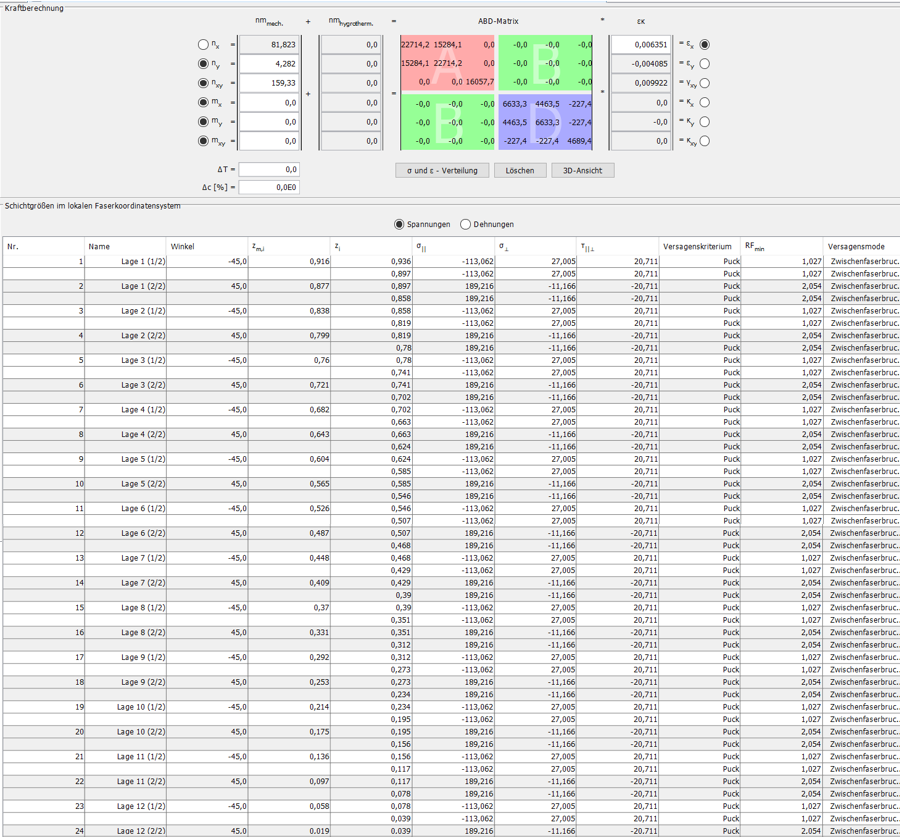
\includegraphics[width=1.0\textwidth]{Bilder/Berechnung Steg dick.png}
	\caption{Berechnung Steg Bereich $I$\&$II$}
	\label{fig:Berechnung Steg dick}
\end{figure}
\begin{figure}
	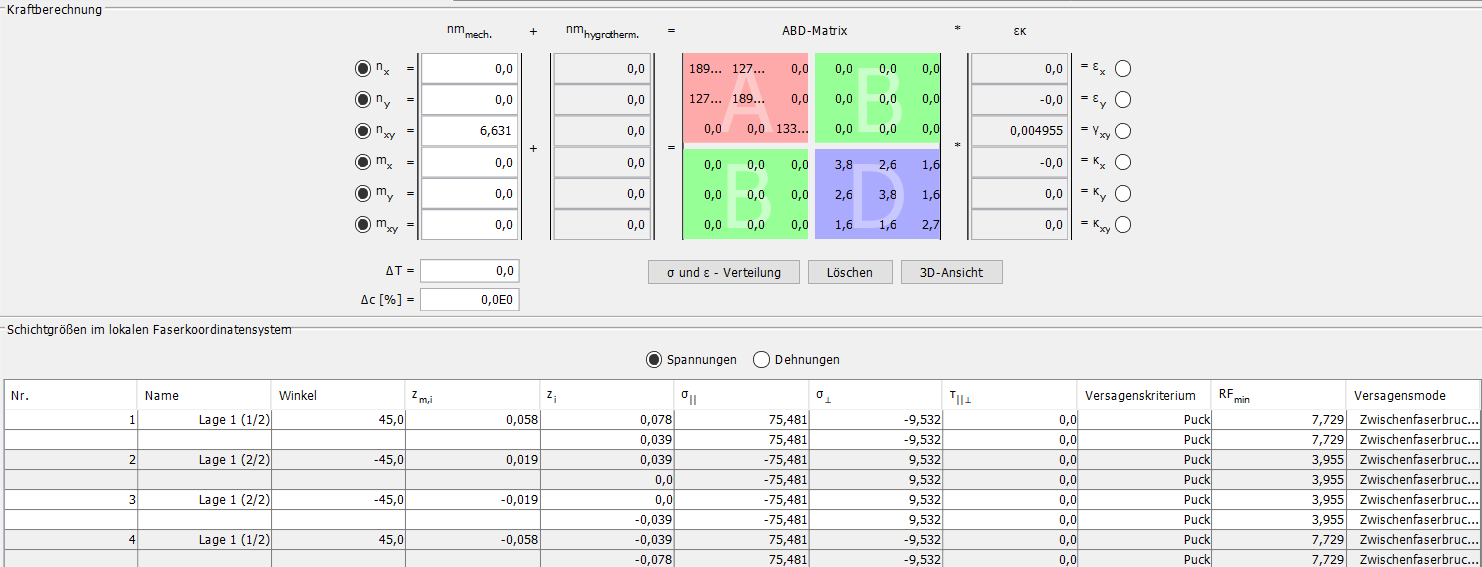
\includegraphics[width=1.0\textwidth]{Bilder/Berechnung Haut.png}
	\caption{Berechnung Flügelschale}
	\label{fig:Berechnung Haut}
\end{figure}
\begin{figure}
	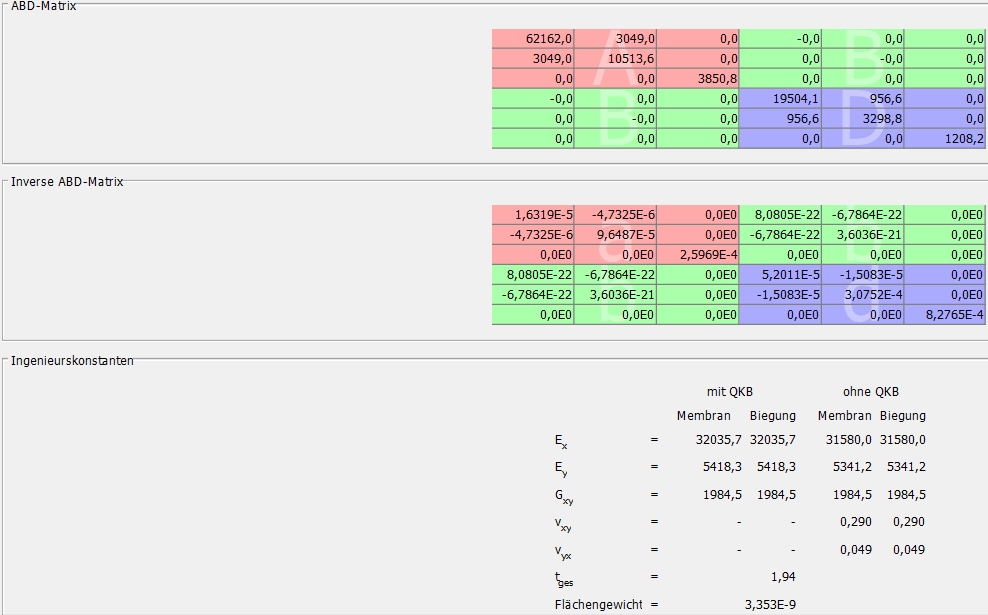
\includegraphics[width=1.0\textwidth]{Bilder/Konstanten Holmgurte.png}
	\caption{Ingenieurskonstanten Holmgurte}
	\label{fig:Ingenieurskonstanten Holmgurte}
\end{figure}
\begin{figure}
	\includegraphics[width=1.0\textwidth]{Bilder/Konstanten Steg dünn.png}
	\caption{BerechnIngenieurskonstantenung Steg Bereich $III$}
	\label{fig:Ingenieurskonstanten Steg dünn}
\end{figure}
\begin{figure}
	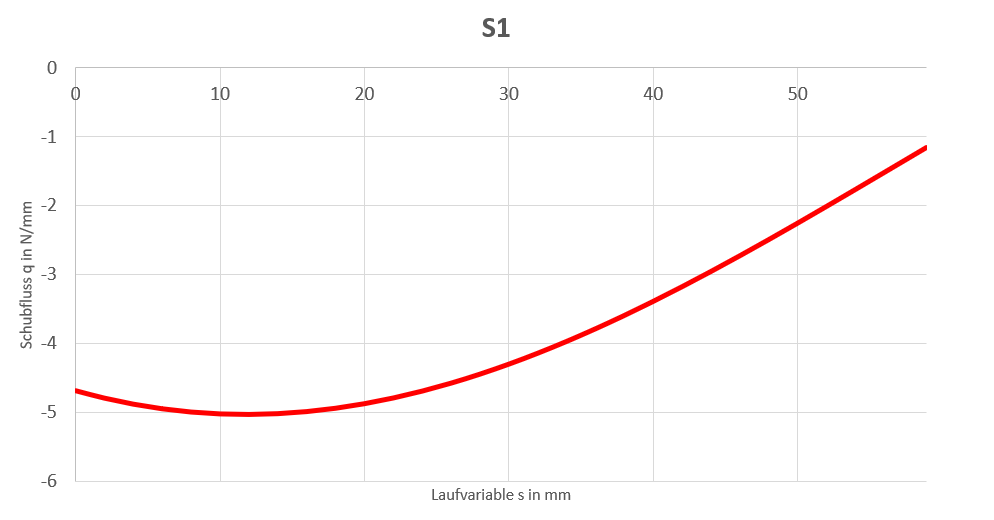
\includegraphics[width=1.0\textwidth]{Bilder/S1.png}
	\caption{Schubfluss Bereich 1}
	\label{fig:S1}
\end{figure}
\begin{figure}
	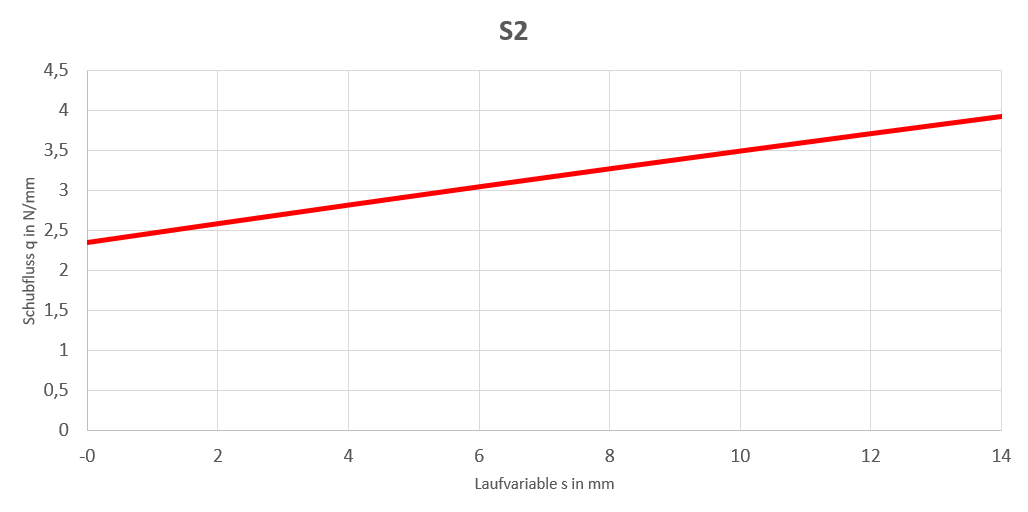
\includegraphics[width=1.0\textwidth]{Bilder/S2.png}
	\caption{Schubfluss Bereich 2}
\end{figure}
\begin{figure}
	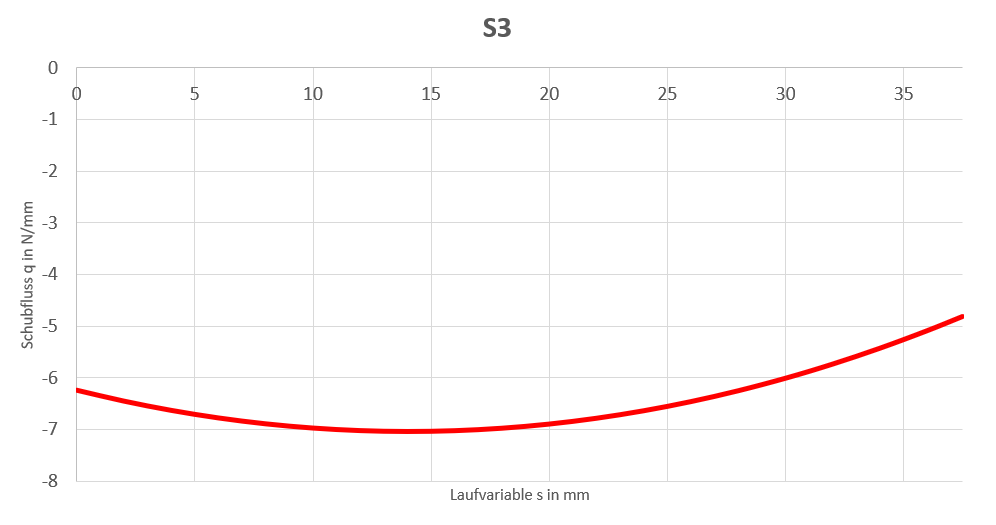
\includegraphics[width=1.0\textwidth]{Bilder/S3.png}
	\caption{Schubfluss Bereich 3}
\end{figure}
\begin{figure}
	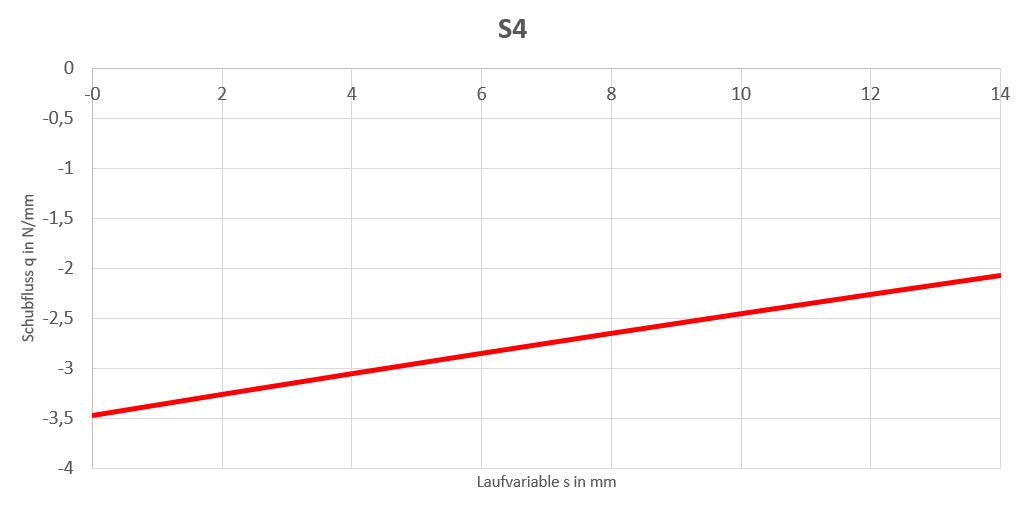
\includegraphics[width=1.0\textwidth]{Bilder/S4.png}
	\caption{Schubfluss Bereich 4}
	\label{fig:S4}
\end{figure}
\begin{figure}
	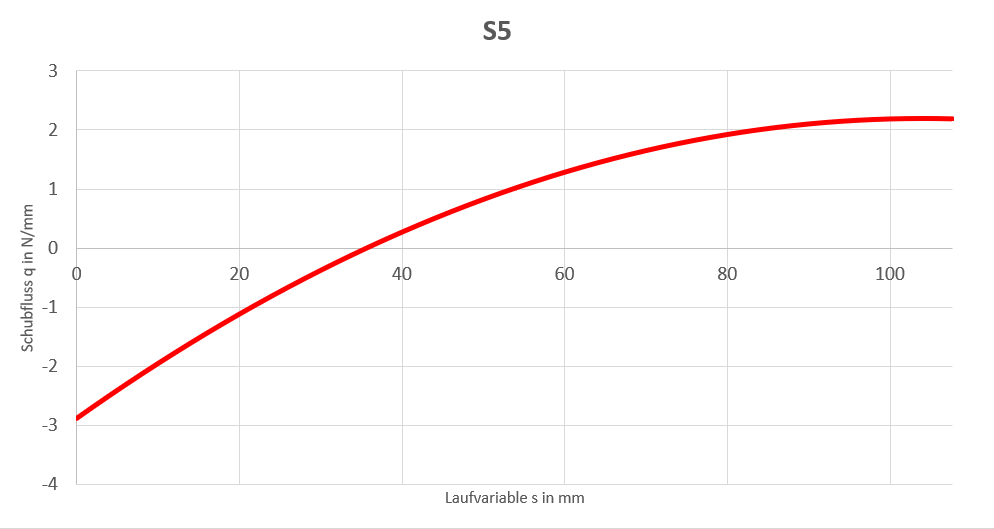
\includegraphics[width=1.0\textwidth]{Bilder/S5.png}
	\caption{Schubfluss Bereich 5}
\end{figure}
\begin{figure}
	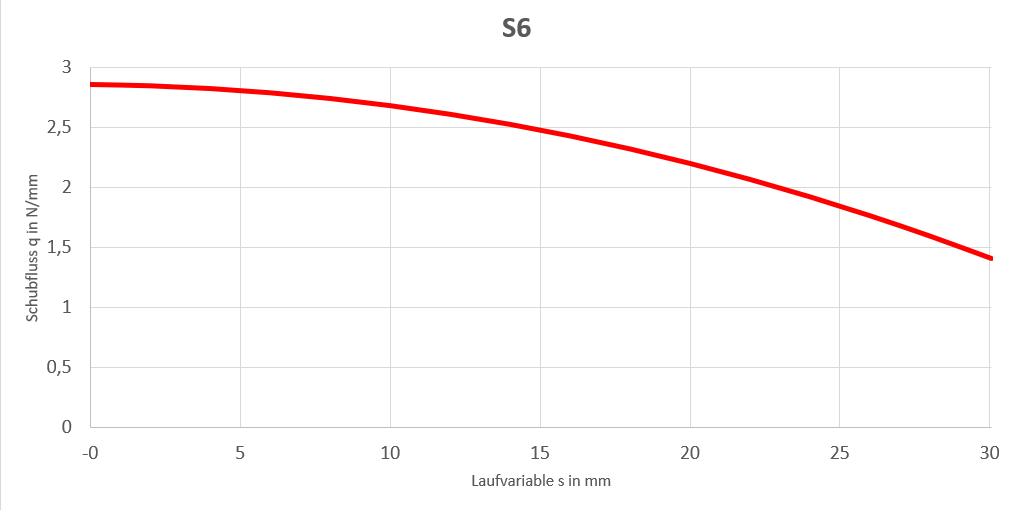
\includegraphics[width=1.0\textwidth]{Bilder/S6.png}
	\caption{Schubfluss Bereich 6}
\end{figure}
\begin{figure}
	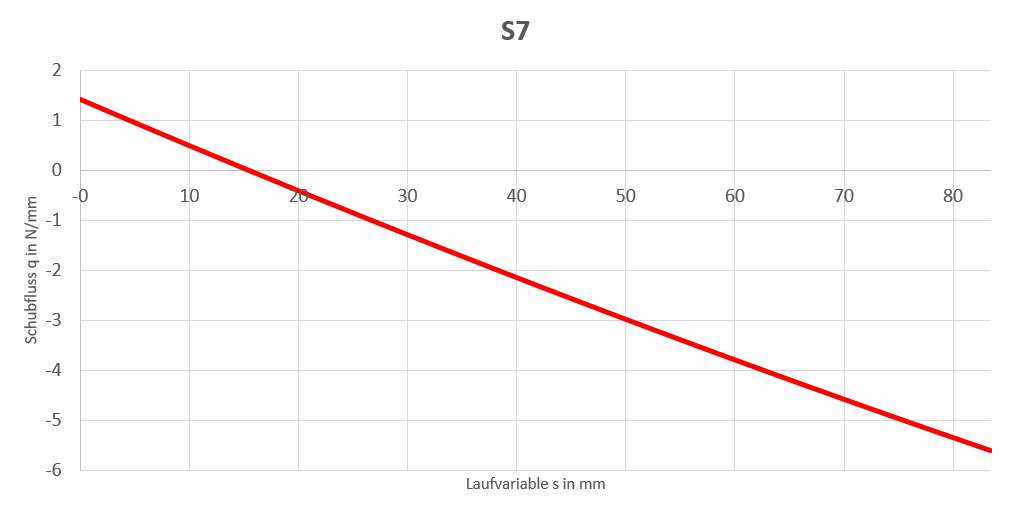
\includegraphics[width=1.0\textwidth]{Bilder/S7.png}
	\caption{Schubfluss Bereich 7}
\end{figure}
\begin{figure}
	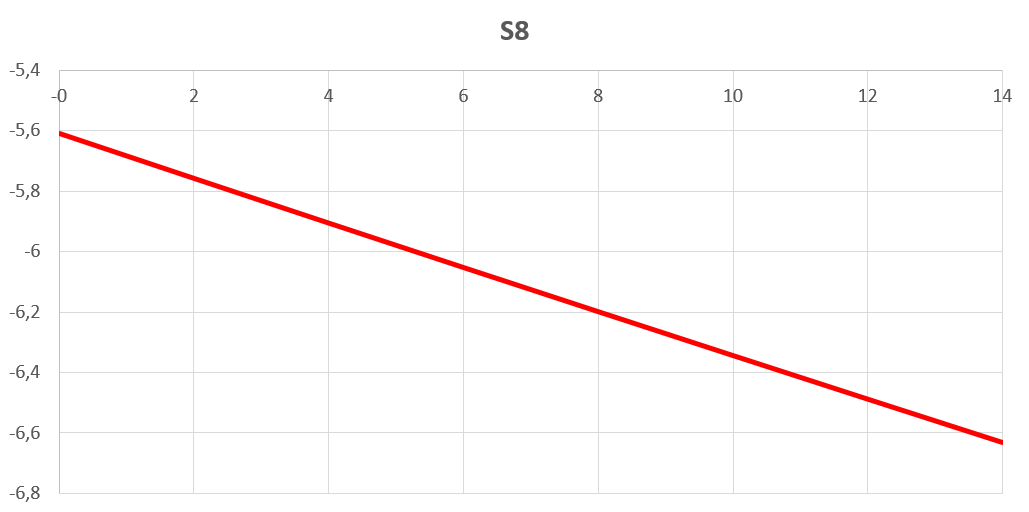
\includegraphics[width=1.0\textwidth]{Bilder/S8.png}
	\caption{Schubfluss Bereich 8}
\end{figure}
\begin{figure}
	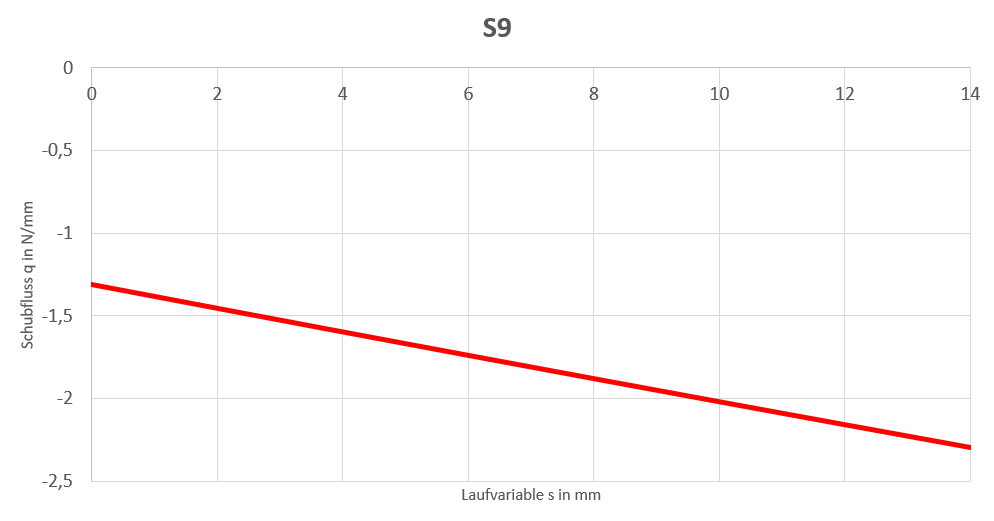
\includegraphics[width=1.0\textwidth]{Bilder/S9.png}
	\caption{Schubfluss Bereich 9}
\end{figure}
\begin{figure}
	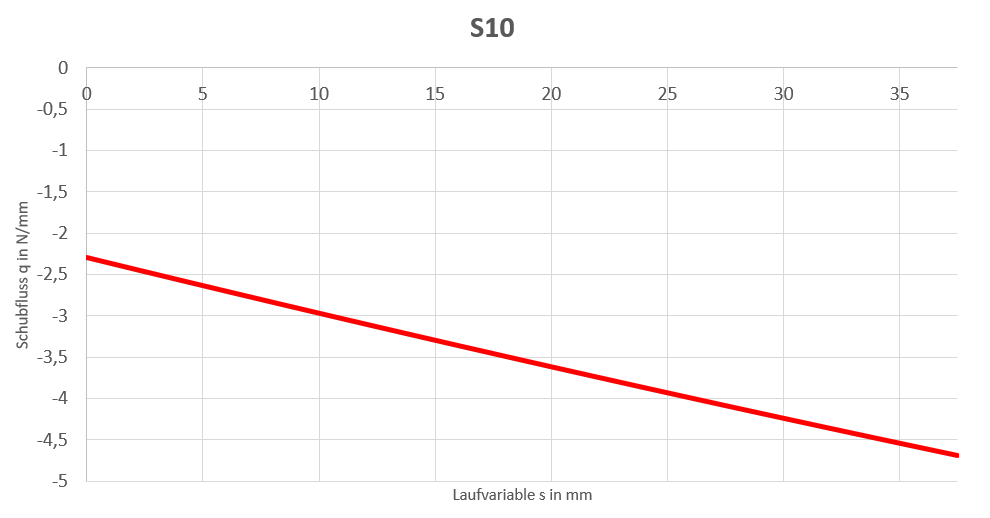
\includegraphics[width=1.0\textwidth]{Bilder/S10.png}
	\caption{Schubfluss Bereich 10}
	\label{fig:S10}
\end{figure}
\begin{figure}
	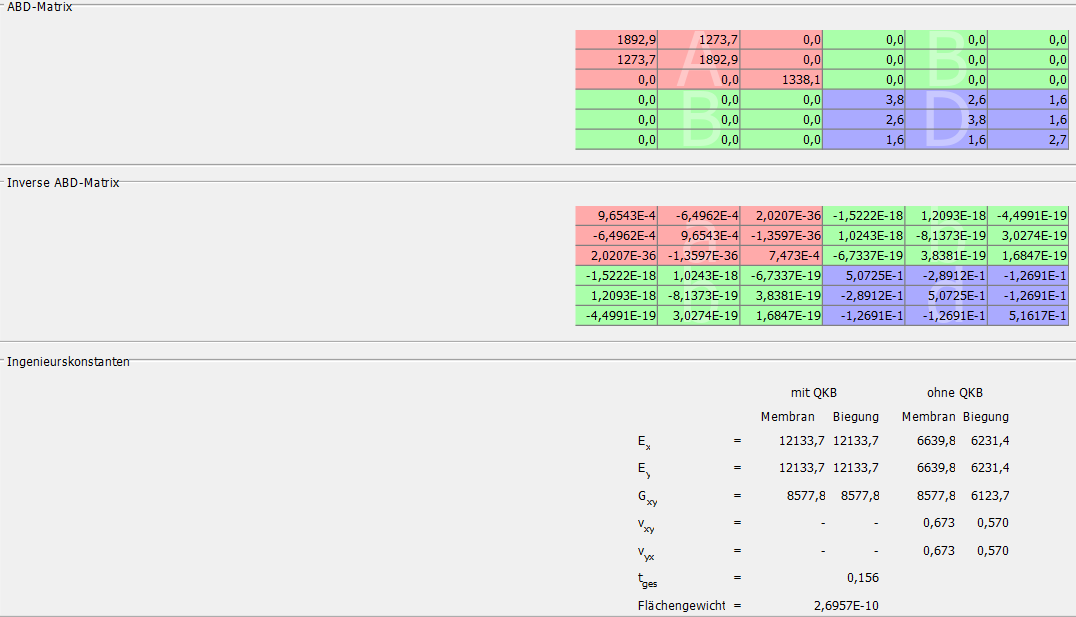
\includegraphics[width=1.0\textwidth]{Bilder/Konstanten Haut.png}
	\caption{Ingenieurskonstanten Flügelschale}
	\label{fig:Ingenieurskonstanten Haut}
\end{figure}
